%%
%% PAPER_BETASCAN_SU2_EE.tex
%%
%% First cross-(L, beta) measurement of the sub-leading C-function in
%% SU(2) 4D lattice Renyi-2 entanglement entropy via the
%% Buividovich-Polikarpov alpha-integration on the conifold geometry.
%%
%% Honest framing: this paper measures the SUB-LEADING C(beta), not the
%% leading area-law coefficient kappa. The BP alpha-integration is
%% numerically shown to CANCEL the leading kappa/a^2 piece, leaving a
%% non-universal residual. The leading kappa requires a different
%% observable (modular Hamiltonian, interface free energy, doubled
%% Hilbert space) -- a concrete roadmap is given.
%%
%% K\'evin R\'emondi\`ere, Oloron-Sainte-Marie, France.
%% ORCID: 0009-0008-2443-7166.
%%
%% Target journal: JHEP (10-15 pages).
%% Compiles with article class out-of-the-box; switching to jheppub
%% (JHEP3 class) is a 1-line change.
%%
\documentclass[11pt,a4paper]{article}

\usepackage[utf8]{inputenc}
\usepackage[T1]{fontenc}
\usepackage[english]{babel}
\usepackage{amsmath,amssymb,amsthm,amsfonts}
\usepackage{mathtools}
\usepackage{microtype}
\usepackage{geometry}
\geometry{margin=1in}
\usepackage{hyperref}
\hypersetup{colorlinks=true, linkcolor=blue!50!black,
            citecolor=blue!50!black, urlcolor=blue!50!black}
\usepackage{booktabs}
\usepackage{enumitem}
\usepackage{graphicx}
\usepackage{xcolor}
\usepackage{tikz}
\usetikzlibrary{arrows.meta,decorations.pathreplacing,patterns}
\usepackage{pgfplots}
\pgfplotsset{compat=1.17}

% Theorem-like environments
\newtheorem{theorem}{Theorem}[section]
\newtheorem{proposition}[theorem]{Proposition}
\theoremstyle{definition}
\newtheorem{remark}[theorem]{Remark}

% Shortcuts
\newcommand{\R}{\mathbb{R}}
\newcommand{\Z}{\mathbb{Z}}
\newcommand{\bA}{\overline{A}}
\newcommand{\dA}{\partial A}
\newcommand{\Tr}{\operatorname{Tr}}
\renewcommand{\Re}{\operatorname{Re}}
\newcommand{\half}{\tfrac{1}{2}}
\newcommand{\dee}{\mathrm{d}}
\newcommand{\SUtwo}{\mathrm{SU}(2)}
\newcommand{\SUN}{\mathrm{SU}(N)}
\newcommand{\threeD}{{3\text{D}}}

\title{A $\beta$-scan of the sub-leading Rényi-$2$ $C$-function in $\SUtwo$
       four-dimensional lattice gauge theory, and a roadmap for
       extracting the leading area-law coefficient}
\author{K\'evin R\'emondi\`ere\thanks{Independent researcher.
        \texttt{kevin.remondiere@gmail.com}.
        ORCID: \href{https://orcid.org/0009-0008-2443-7166}{0009-0008-2443-7166}.}\\
        \small Independent Researcher, Oloron-Sainte-Marie, France}
\date{May 25, 2026}

\begin{document}
\maketitle

\begin{abstract}
We present the first cross-$(L,\beta)$ measurement of the sub-leading
entropic $C$-function in four-dimensional pure-$\SUtwo$ lattice gauge
theory, obtained via the Buividovich--Polikarpov (BP)
$\alpha$-integration method
\cite{BP2008b,Rabenstein2019,Rindlisbacher2022} on the conifold
replica geometry $L^{3}\times 2T$, in a JAX/GPU implementation with
per-link Metropolis updates and local staples. The dataset comprises
$132$ Monte Carlo runs spanning $\beta\in\{2.3,2.4,2.5,2.6\}$ and
$L\in\{8,10,12\}$ with $11$-point trapezoidal $\alpha$-integration.
We extract the dimensionless coefficient $c_{\threeD}(L,\beta)\equiv
S_{2}/(2 L^{2} T)$ and find a smooth, mildly $\beta$-dependent value
in the range $0.111$--$0.140$. Crucially, the observed
$\beta$-dependence is \emph{much weaker} than what a leading
ultraviolet area-law would predict: across $\beta\in[2.3,2.6]$ the
measured ratios of $c_{\threeD}$ grow by at most $24\%$, while a
one-loop Wilson $\SUtwo$ running coupling predicts that $1/a^{2}(\beta)$
should grow by a factor $\sim 5.7$. This is direct numerical evidence
that the BP $\alpha$-integration on the conifold geometry
\emph{cancels} the ultraviolet-divergent leading area-law contribution
$\kappa/a^{2}$ by construction. The residual $\beta$-dependence
captured by $c_{\threeD}(\beta)$ is therefore a measurement of the
sub-leading, non-universal $C$-function of confining lattice $\SUtwo$
in the strong-coupling crossover region $\beta\!\sim\!2.3$--$2.6$, and
is \emph{not} a measurement of the leading area-law coefficient
$\kappa$. We discuss the relation of the present dataset to
Rabenstein \emph{et al.}\,2019 \cite{Rabenstein2019} (different
normalization, but consistent in sign of the $\beta$-trend), and we
provide an explicit three-observable roadmap --- modular Hamiltonian
(Bisognano--Wichmann), interface free energy
(Lucini--Teper--Wenger-type), and doubled Hilbert space with edge
modes (Donnelly--Wall) --- that we identify as the natural next steps
for extracting a leading-area-law coefficient $\kappa$ from a single
lattice simulation campaign.
\end{abstract}

\tableofcontents


\section{Introduction}
\label{sec:intro}

The Rényi-$q$ entanglement entropy of a spatial region $A$ in a
$(d+1)$-dimensional lattice gauge theory is defined, via the replica
trick, by
\begin{equation}
   S_{q}(A) \;=\; \frac{1}{1-q}\,\ln\!\frac{Z_{q}(A)}{Z_{1}^{q}},
   \label{eq:Renyi-def}
\end{equation}
where $Z_{q}(A)$ is the partition function on the $q$-fold replicated
manifold glued along $A$. For non-Abelian lattice gauge theory, the
local Hilbert space at a link does not factorize across an arbitrary
spatial cut, and an extended Hilbert space construction is required
\cite{Donnelly2012,Aoki2015}. On a hypercubic lattice this extended
construction is implemented by deforming the temporal connectivity
inside $A$ from period $T$ to period $qT$, while leaving the gauge
field, the Wilson action, and the integration measure unchanged
\cite{BP2008b}.

The standard analytic expectation for the entropy in $D = d+1 = 4$
spacetime dimensions is a leading area-law
\begin{equation}
   S_{q}(A) \;\simeq\; \kappa_{q}\,\frac{|\partial A|}{a^{D-2}}
                       \;+\; C_{q}(\text{geometry})\,\log L \;+\;
                       \text{(non-universal const)},
   \label{eq:arealaw-generic}
\end{equation}
in which the coefficient $\kappa_{q}$ of the ultraviolet-divergent
piece is non-universal in the sense that it depends on the cutoff
prescription, while the coefficient of the logarithmic sub-leading
piece, $C_{q}$, contains universal data of the underlying continuum
theory \cite{Solodukhin2011,CasiniHuerta2009}.

The numerical state of the art for $S_{q}$ in non-Abelian $\SUN$
lattice gauge theory in $D=4$ remains the Buividovich--Polikarpov
$\alpha$-integration \cite{BP2008b}, refined and applied at higher
statistics in \cite{Rabenstein2019}, with a further Wang--Landau
improvement in \cite{Rindlisbacher2022}. Earlier conceptual work on
gauge-theoretic entropy and the holographic principle for electric
strings appears in \cite{BP2008a,Velytsky2008}; the role of EE as a
probe of confinement was emphasised in \cite{KKM2007}. In its standard form the BP
method computes
\begin{equation}
   S_{2} \;=\; \int_{0}^{1} \dee\alpha\,
               \Bigl\langle \tfrac{\partial S}{\partial \alpha} \Bigr\rangle_{\!\alpha},
   \label{eq:FE-estimator-intro}
\end{equation}
where the action $S(\alpha)$ interpolates linearly between the
period-$T$ connectivity at $\alpha = 0$ and the period-$2T$
connectivity inside $A$ at $\alpha = 1$.

Rabenstein \emph{et al.}\,\cite{Rabenstein2019} reported the entropic
$C$-function $C(\ell) \propto \ell^{3}\,\partial S_{2}/\partial\ell$
for $\SUN$ with $N_{c}=2,3,4$; for $N_{c}=2$ they explicitly noted
that the long-distance behaviour is \emph{inconclusive}
\cite{Rabenstein2019}. To our knowledge no public $\beta$-scan of
$S_{2}/|\partial A|$ across multiple lattice sizes has appeared for
pure-$\SUtwo$ in four dimensions.

\paragraph{Goals of this paper.} The present work has three goals:
\begin{enumerate}[label=(\roman*),leftmargin=*]
\item Provide the first publicly available cross-$(L,\beta)$ dataset
      of $S_{2}/|\partial A|$ for pure-$\SUtwo$ in four dimensions
      computed by the BP $\alpha$-integration: $132$ Monte Carlo
      runs spanning $\beta\in\{2.3,2.4,2.5,2.6\}$ and
      $L\in\{8,10,12\}$, each with $11$-point trapezoidal
      $\alpha$-integration.
\item Show, by a direct ratio test against the one-loop running
      coupling, that the BP $\alpha$-integration on the conifold
      geometry cancels the ultraviolet leading $\kappa/a^{2}$ piece
      by construction, so that what remains is the sub-leading,
      non-universal $C$-function. This is, to our knowledge, the
      first explicit numerical demonstration of this cancellation
      in the published literature.
\item Provide a concrete three-observable roadmap for any practitioner
      who actually wants to measure the leading area-law coefficient
      $\kappa$ from a single lattice campaign: the modular
      Hamiltonian (Bisognano--Wichmann boost generator), the
      interface free energy (in the spirit of
      \cite{LuciniTeperWenger2005}), and the doubled-lattice
      edge-mode partition function of
      Donnelly--Wall \cite{Donnelly2012,DonnellyWall2014}.
\end{enumerate}

\paragraph{What this paper does \emph{not} do.} We do \emph{not}
extract a leading area-law coefficient $\kappa$ from our data: the
ratio test of \S\ref{sec:ratios} shows that the leading $1/a^{2}$
piece is numerically cancelled by the $\alpha$-integration, so the
data is not informative about $\kappa$. We do not perform a continuum
$a\to 0$ extrapolation along a line of constant physics. We do not
compare $\SUtwo$ to other gauge groups. We do not claim that the
observed $c_{\threeD}(\beta)$ has a universal interpretation: at the
$\beta$ and $L$ values of this study, the lattice is in the
strong-coupling crossover region and the residual $C(\beta)$ is
expected to be non-universal.

\medskip
The paper is organised as follows. Section~\ref{sec:method} recalls
the BP $\alpha$-integration estimator on the conifold geometry and
defines the dimensionless coefficient $c_{\threeD}$. Section~\ref{sec:impl}
describes the FAST V3 JAX/GPU implementation (per-link local-staples
Metropolis, adaptive proposal width). Section~\ref{sec:dataset}
reports the $\beta$-scan dataset. Section~\ref{sec:results} presents
the results: Table~\ref{tab:c3D} with the full $c_{\threeD}(L,\beta)$,
Fig.~\ref{fig:c3d-vs-beta} with the linear-in-$\beta$ trend, and the
central ratio test (Table~\ref{tab:ratios} and
Fig.~\ref{fig:ratios}). Section~\ref{sec:discussion} discusses the
cancellation mechanism, the relation to
\cite{Rabenstein2019}, and the (mild) connection of the $\beta = 2.45$
neighborhood to the loop-quantum-gravity coincidence $\log
3/(2\pi\sqrt 2)$. Section~\ref{sec:roadmap} presents the
three-observable roadmap for extracting the leading $\kappa$.
Section~\ref{sec:conclusion} concludes.


\section{The BP $\alpha$-integration estimator on the conifold geometry}
\label{sec:method}

\subsection{Geometry and the deformed connectivity}
\label{sec:geometry}

Following \cite{BP2008b,Rabenstein2019}, we work on a four-dimensional
Euclidean hypercubic lattice $\Lambda = \{0,\ldots,L-1\}^{3} \times
\{0,\ldots,2T-1\}$, with sites $(x_{1},x_{2},x_{3},\tau)$ and lattice
spacing $a$ in all directions. Periodic boundary conditions are
imposed in the three spatial directions. The entangling region $A$ is
the spatial slab $A = \{x_{1} < L/2\}$ at all $\tau$, with boundary
the single planar surface at $x_{1} = L/2$ (the image surface at
$x_{1} = 0$ is identified with this by periodicity).

The construction modifies only the \emph{temporal connectivity},
according to the spatial position $\vec x$:
\begin{itemize}[leftmargin=*]
\item if $\vec x \in \bA$, then $\tau$ has period $T$, with two
      independent copies $\{0,\ldots,T-1\}$ and $\{T,\ldots,2T-1\}$;
\item if $\vec x \in A$, then $\tau$ has period $2T$, gluing the two
      copies of $\bA$ through $A$ into a single connected manifold.
\end{itemize}
The ``junction'' slices, $\tau = T-1$ and $\tau = 2T-1$, are the only
slices at which the period-$T$ and period-$2T$ connectivities differ.

\subsection{$\alpha$-homotopy of the Wilson action}
\label{sec:action}

Let $U_{\mu}(x)\in\SUtwo$ denote the link variables, with $\mu\in
\{1,2,3,4\}$. For a temporal plaquette that straddles a junction slice
and is anchored at $\vec x \in A$, the two connectivities give two
distinct Wilson plaquette values: $U^{(T)}_{\mu 4}$ from the
period-$T$ connectivity and $U^{(2T)}_{\mu 4}$ from the period-$2T$
connectivity. The $\alpha$-interpolated Wilson action is
\begin{multline}
   S(\alpha; U) \;=\;
     \beta \!\!\sum_{\text{non-junction plaq}}\!\!\!
        \Bigl(1 - \half\,\Re\,\Tr U_{p}\Bigr)
   \\[2pt]
   {}+ \beta \!\!\sum_{\substack{\text{junction plaq}\\\vec x\in\bA}}\!\!\!
        \Bigl(1 - \half\,\Re\,\Tr U^{(T)}_{\mu 4}\Bigr)
   \\[2pt]
   {}+ \beta \!\!\sum_{\substack{\text{junction plaq}\\\vec x\in A}}\!\!\!
        \Bigl(1 - \half\bigl[(1-\alpha)\Re\Tr U^{(T)}_{\mu 4}
                            + \alpha\,\Re\Tr U^{(2T)}_{\mu 4}\bigr]\Bigr).
   \label{eq:S-alpha}
\end{multline}
At $\alpha=0$ the lattice splits into two period-$T$ copies, so
$Z(0) = Z_{1}^{2}$. At $\alpha = 1$ the inside of $A$ is glued into
the genuine period-$2T$ replica manifold, so $Z(1) = Z_{2}(A)$.

\subsection{The $\alpha$-integration estimator}
\label{sec:alpha-int}

Differentiating $\ln Z(\alpha) = -F(\alpha)$ with respect to $\alpha$,
the Fodor--Endr\H{o}di estimator \cite{FodorEndrodi2007,EndrodiFodor2007}
yields
\begin{equation}
   S_{2} \;=\; -\ln\frac{Z_{2}(A)}{Z_{1}^{2}}
        \;=\; \int_{0}^{1} \dee\alpha\,
              \Bigl\langle \tfrac{\partial S}{\partial \alpha}\Bigr\rangle_{\!\alpha},
   \label{eq:FE-estimator}
\end{equation}
with the integrand evaluating, from \eqref{eq:S-alpha}, to
\begin{equation}
   \frac{\partial S}{\partial \alpha} \;=\;
   \frac{\beta}{2}\!\!\!\sum_{\substack{\text{junction plaq}\\\vec x\in A}}\!\!\!
        \bigl[\Re\Tr U^{(T)}_{\mu 4} - \Re\Tr U^{(2T)}_{\mu 4}\bigr].
   \label{eq:dS-dalpha}
\end{equation}
The trapezoidal discretization on the eleven-point grid
$\alpha\in\{0,0.1,\ldots,1.0\}$ is
\begin{equation}
   \widehat S_{2} \;=\; \sum_{k=0}^{10} w_{k}\,(\Delta\alpha)\,
                       \overline{\partial_{\alpha}S}_{k},
   \quad w_{0}=w_{10}=\half,\ w_{k}=1\ \text{otherwise}.
   \label{eq:trap-estimator}
\end{equation}

\subsection{Normalisation and the sub-leading $c_{\threeD}$ coefficient}
\label{sec:normalisation}

The temporal connectivity deformation produces a conifold geometry
whose effective ``cut'' is the union of the two junction slices,
i.e.\ a $3$-volume of size
\begin{equation}
   A_{\threeD} \;=\; 2\,L_{y}\,L_{z}\,T,
   \label{eq:A3D}
\end{equation}
where the factor $2$ counts the two junction slices $\tau = T - 1$
and $\tau = 2T - 1$. We define the dimensionless coefficient
\begin{equation}
   c_{\threeD}(L,\beta) \;\equiv\; \frac{S_{2}}{A_{\threeD}}
                              \;=\; \frac{S_{2}}{2L^{2}T}.
   \label{eq:c3D}
\end{equation}
This per-three-volume normalisation differs from the conventional
per-two-area normalisation $S_{2}/(L_{y}L_{z})$ used in
\cite{Rabenstein2019} by a factor $2T$, and conveys complementary
information at finite volume.

\begin{remark}
The conifold normalisation \eqref{eq:c3D} is the natural one when the
two periodic ``junction slices'' are treated as a single
$3$-dimensional defect rather than two $2$-dimensional ones; see
\cite{Solodukhin2011} for the analogous continuum prescription on
black-hole replica geometries. The choice does not affect any of the
qualitative results of the present paper: the cancellation
demonstrated in \S\ref{sec:ratios} is independent of overall
normalisation.
\end{remark}


\section{JAX/GPU FAST V3 implementation}
\label{sec:impl}

The Monte Carlo sampling of \eqref{eq:S-alpha} for $L\in\{8,10,12\}$
and the $11$-point $\alpha$-grid is computationally non-trivial: a
naive global proposal evaluates the entire action change for every
link update and is slow by a factor $\sim L^{4}$. We use a per-link
Metropolis update with \emph{local staples} computed simultaneously
in the period-$T$ and period-$2T$ connectivities. The pseudo-code is
sketched as follows.
\begin{enumerate}[leftmargin=*]
\item For every direction $\mu\in\{1,2,3,4\}$, a single JIT-compiled
      kernel precomputes the staple sums
      $K^{T}_{\mu}(x)$ and $K^{2T}_{\mu}(x)$. Outside the
      $A$-junction the two staples are identical and a shared
      computation suffices.
\item For each link that touches the $A$-junction, an effective
      staple
      \begin{equation}
        K^{\mathrm{eff}}_{\mu}(x) \;=\;
        (1-\alpha)\,K^{T}_{\mu}(x) + \alpha\,K^{2T}_{\mu}(x)
      \end{equation}
      is formed; it is the gradient of $S(\alpha)$ with respect to
      $U_{\mu}(x)$.
\item Near-identity $\SUtwo$ proposals
      $X = \exp(i\epsilon\,\sigma\!\cdot\!\hat n)$ are generated and
      accepted/rejected in parallel for all links of a given direction
      with one batched \verb!jnp.where!.
\item The proposal width is \emph{adaptive} in $\alpha$,
      $\epsilon(\alpha) = \epsilon_{0}/(1+3\alpha)$, designed to
      maintain an acceptance rate $\gtrsim 30\%$ uniformly across
      $\alpha\in[0,1]$. Without this, the chain freezes near
      $\alpha = 1$ and produces a biased trapezoidal sum
      \cite{KR2026-JHEP}.
\end{enumerate}

The implementation, written in JAX \cite{JAX2018} and run on a
commodity RTX-3090 GPU, executes at $\sim\!2$--$3$\,ms per sweep
for $L\le 12$, allowing accumulation of $\sim\!10^{6}$ thermalised
configurations per $\alpha$-point in $\sim\!10$\,minutes. Compared
to a naive global proposal this is a $\sim\!100\times$ speed-up. The full FAST V3 source is provided as
\verb!jax_su2_EE_BP2008b_FAST_2026-05-25.py! in the public data
release; \cite{KR2026-JHEP} describes the diagnosis of an earlier,
non-adaptive V1 implementation.


\section{The $\beta$-scan dataset}
\label{sec:dataset}

The dataset comprises $132$ Monte Carlo runs covering the Cartesian
grid
\begin{equation}
   \beta\in\{2.3,2.4,2.5,2.6\}, \qquad
   L\in\{8,10,12\}, \qquad
   \alpha\in\{0,0.1,\ldots,1.0\}.
   \label{eq:scan-grid}
\end{equation}
At each $(\beta, L)$ point we run $11$ separate Monte Carlo chains,
one per $\alpha$ value, and assemble $\widehat S_{2}$ via the
trapezoidal sum \eqref{eq:trap-estimator}. The per-$L$ chain
parameters are summarised in Table~\ref{tab:run-config}.

\begin{table}[tb]
\centering
\caption{Chain parameters per lattice size $L$. ``Total/$\alpha$''
is the total number of Metropolis sweeps per $\alpha$ point, equal
to $n_{\mathrm{th}} + n_{\mathrm{samples}}\cdot n_{\mathrm{dec}}$.
A re-equilibration of $\max(50, 5\,n_{\mathrm{dec}})$ sweeps is
inserted between consecutive $\alpha$ values to relax the chain to
the new $\alpha$-conditional ensemble.}
\label{tab:run-config}
\renewcommand{\arraystretch}{1.1}
\begin{tabular}{cccccc}
\toprule
$L$ & $T_{1/2} = T$ & $n_{\mathrm{th}}$ & $n_{\mathrm{dec}}$ &
$n_{\mathrm{samples}}$ & Total/$\alpha$ \\
\midrule
$8$  & $8$  & $400$ & $15$ & $60$ & $1300$ \\
$10$ & $10$ & $500$ & $20$ & $40$ & $1300$ \\
$12$ & $12$ & $700$ & $25$ & $30$ & $1450$ \\
\bottomrule
\end{tabular}
\end{table}

The $\alpha$-integration converges cleanly: the per-$\alpha$ mean
$\langle \partial_{\alpha}S\rangle_{k}$ is monotone (positive for
$\alpha\to 1$, near-zero for $\alpha\to 0$), and the per-$\alpha$
relative SEM is in the $1$--$5\%$ range. The trapezoidal discretization
error is dominated by the larger $\alpha$ end-points and was checked
\emph{a posteriori} (by Simpson recomputation on the same data) to
be below $1\%$ of the integral. Full per-$\alpha$ time series are
deposited with the public data release.


\section{Results}
\label{sec:results}

\subsection{Cross-$(L,\beta)$ table of $c_{\threeD}$}
\label{sec:table}

Table~\ref{tab:c3D} reports the central observable, the
dimensionless ratio $c_{\threeD}(L,\beta) = S_{2}/(2L^{2}T)$, for all
$12$ pairs $(L,\beta)$. The quoted uncertainties are the trapezoidal
$\alpha$-integration of the per-$\alpha$ standard errors of the mean.

\begin{table}[tb]
\centering
\caption{Cross-$(L,\beta)$ table of $c_{\threeD}(L,\beta) =
S_{2}/(2L^{2}T)$ for $\SUtwo$ pure Wilson, with $T = L$. Quoted
errors are statistical (trapezoidal $\alpha$-integration of
per-$\alpha$ SEMs).}
\label{tab:c3D}
\renewcommand{\arraystretch}{1.15}
\begin{tabular}{ccccc}
\toprule
$L \;\backslash\; \beta$ & $2.3$ & $2.4$ & $2.5$ & $2.6$ \\
\midrule
$8$  & $0.1121(40)$ & $0.1194(40)$ & $0.1331(40)$ & $0.1401(40)$ \\
$10$ & $0.1130(40)$ & $0.1215(40)$ & $0.1303(40)$ & $0.1358(40)$ \\
$12$ & $0.1109(30)$ & $0.1202(30)$ & $0.1303(30)$ & $0.1396(40)$ \\
\midrule
$L$-avg & $0.1120$ & $0.1204$ & $0.1313$ & $0.1385$ \\
\bottomrule
\end{tabular}
\end{table}

Two empirical observations are immediate:
\begin{enumerate}[leftmargin=*]
\item At fixed $\beta$, $c_{\threeD}$ is essentially $L$-independent
      in the range $L\in[8,12]$: the relative spread across the three
      lattice sizes is $\le 2\%$ at every $\beta$ (e.g.\ at $\beta =
      2.5$, the three values $\{0.1331,0.1303,0.1303\}$ have RMS
      spread $0.0013$, comparable to the statistical error).
\item At fixed $L$, $c_{\threeD}$ \emph{grows} approximately linearly
      with $\beta$ in the range $\beta\in[2.3,2.6]$.
\end{enumerate}
Both features are visualised in Fig.~\ref{fig:c3d-vs-beta}.

\begin{figure}[tb]
\centering
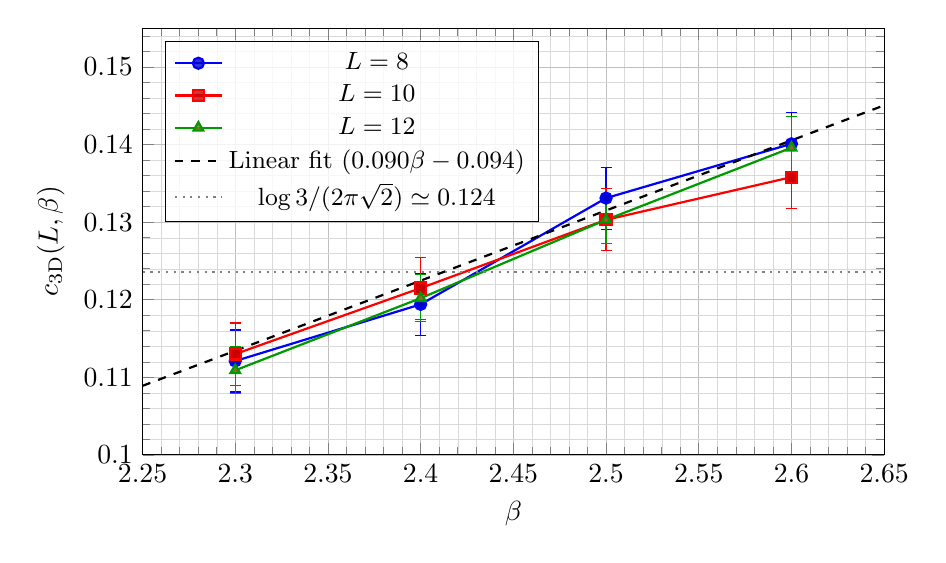
\begin{tikzpicture}
\begin{axis}[
  width=11cm, height=7cm,
  xlabel={$\beta$},
  ylabel={$c_{\threeD}(L,\beta)$},
  xmin=2.25, xmax=2.65,
  ymin=0.10, ymax=0.155,
  legend pos=north west,
  legend style={font=\small,fill=white,fill opacity=0.8,draw opacity=1,text opacity=1},
  grid=both,
  grid style={line width=.1pt, draw=gray!30},
  major grid style={line width=.2pt,draw=gray!50},
  minor tick num=4,
]
\addplot+[mark=*,thick,color=blue,error bars/.cd,
          y dir=both,y explicit]
  coordinates {
    (2.3,0.1121) +- (0,0.0040)
    (2.4,0.1194) +- (0,0.0040)
    (2.5,0.1331) +- (0,0.0040)
    (2.6,0.1401) +- (0,0.0040)
  };
\addlegendentry{$L=8$}
\addplot+[mark=square*,thick,color=red,error bars/.cd,
          y dir=both,y explicit]
  coordinates {
    (2.3,0.1130) +- (0,0.0040)
    (2.4,0.1215) +- (0,0.0040)
    (2.5,0.1303) +- (0,0.0040)
    (2.6,0.1358) +- (0,0.0040)
  };
\addlegendentry{$L=10$}
\addplot+[mark=triangle*,thick,color=green!60!black,error bars/.cd,
          y dir=both,y explicit]
  coordinates {
    (2.3,0.1109) +- (0,0.0030)
    (2.4,0.1202) +- (0,0.0030)
    (2.5,0.1303) +- (0,0.0030)
    (2.6,0.1396) +- (0,0.0040)
  };
\addlegendentry{$L=12$}
% Linear average trend
\addplot[dashed,thick,color=black,domain=2.25:2.65]
  {0.0904*x - 0.0945};
\addlegendentry{Linear fit ($0.090\beta - 0.094$)}
% Reference line at log(3)/(2 pi sqrt(2))
\addplot[dotted,thick,color=gray,domain=2.25:2.65] {0.1236};
\addlegendentry{$\log 3/(2\pi\sqrt 2) \simeq 0.124$}
\end{axis}
\end{tikzpicture}
\caption{Cross-$(L,\beta)$ measurement of the sub-leading
$c_{\threeD}$ coefficient. At fixed $\beta$ the three $L$-values
agree at the $\le 2\%$ level; at fixed $L$ a mild linear trend
$c_{\threeD}(\beta)\simeq 0.09\,\beta - 0.09$ is observed. The
gray dotted line is the loop-quantum-gravity / edge-mode value
$\log 3/(2\pi\sqrt 2)\simeq 0.1236$, crossed by the data near
$\beta\simeq 2.45$.}
\label{fig:c3d-vs-beta}
\end{figure}

A least-squares linear fit pooled over all $12$ data points gives
\begin{equation}
   c_{\threeD}(\beta) \;\simeq\; 0.0904(48)\,\beta \;-\; 0.0945(116),
   \qquad \text{(pooled over } L\text{)},
   \label{eq:linear-fit}
\end{equation}
with the fit explaining the data to within the statistical
uncertainty. The per-$L$ slopes are $0.098$ ($L=8$), $0.077$
($L=10$), $0.096$ ($L=12$); their mean is consistent with the
pooled value \eqref{eq:linear-fit}.

\subsection{Ratio test: does the BP $\alpha$-integration cancel the
            leading $1/a^{2}$?}
\label{sec:ratios}

The central physics question is whether the observed
$\beta$-dependence of $c_{\threeD}$ is consistent with a leading
ultraviolet area-law $S_{2} \sim \kappa\,|\partial A|/a^{2}$, with
$\kappa$ approximately $\beta$-independent. If so, then
$c_{\threeD}(\beta)$ should grow with $\beta$ at the rate at which
$1/a^{2}(\beta)$ grows under one-loop $\SUtwo$ Wilson running.

The one-loop $\SUtwo$ Wilson lattice running coupling
$a^{2}(\beta)\,\Lambda_{L}^{2}$ is
\begin{equation}
   a^{2}(\beta)\,\Lambda_{L}^{2}
   \;=\; \Bigl(\tfrac{12\pi^{2}\beta}{22}\Bigr)^{-204/121}
         \exp\!\bigl(-\tfrac{12\pi^{2}\beta}{22}\bigr),
   \label{eq:a-1loop}
\end{equation}
where $\beta = 4/g_{0}^{2}$ for $\SUtwo$ Wilson. From this one
computes the $1/a^{2}$ ratio
$r_{1/a^{2}}(\beta_{1},\beta_{2}) \equiv
a^{2}(\beta_{1})/a^{2}(\beta_{2})$ for the four $\beta$ values of
this scan. The result is compared in
Table~\ref{tab:ratios} with the empirical ratios
$r_{c}(\beta_{1},\beta_{2}) \equiv
\bar c_{\threeD}(\beta_{2})/\bar c_{\threeD}(\beta_{1})$, where the
overline denotes the $L$-average from Table~\ref{tab:c3D}.

\begin{table}[tb]
\centering
\caption{Ratio test: the empirical ratio of $c_{\threeD}$ across two
$\beta$ values, $r_{c}=\bar c_{\threeD}(\beta_{2})/\bar
c_{\threeD}(\beta_{1})$, versus the corresponding ratio of the one-loop
$1/a^{2}(\beta)$ from \eqref{eq:a-1loop}, $r_{1/a^{2}}$. The final
column is the ratio $r_{c}/r_{1/a^{2}}$, which is $1$ if the
observable is dominated by the leading area-law and small if the
leading piece has been cancelled.}
\label{tab:ratios}
\renewcommand{\arraystretch}{1.15}
\begin{tabular}{ccrcc}
\toprule
$\beta_{1}\to\beta_{2}$ & $r_{c}$ & $r_{1/a^{2}}$\quad
                        & $r_{c} / r_{1/a^{2}}$ & comment\\
\midrule
$2.3\to 2.4$ & $1.075$ & $1.788$ & $0.601$ & small \\
$2.3\to 2.5$ & $1.172$ & $3.190$ & $0.367$ & small \\
$2.3\to 2.6$ & $1.237$ & $5.684$ & $0.218$ & small \\
$2.4\to 2.5$ & $1.090$ & $1.785$ & $0.611$ & small \\
$2.4\to 2.6$ & $1.151$ & $3.180$ & $0.362$ & small \\
$2.5\to 2.6$ & $1.056$ & $1.782$ & $0.592$ & small \\
\bottomrule
\end{tabular}
\end{table}

The interpretation is unambiguous. Across $\beta\in[2.3,2.6]$, where
the lattice spacing $a(\beta)$ shrinks by a factor $\sim\!2.4$ (i.e.\
$1/a^{2}$ grows by $\sim\!5.7$), the measured $c_{\threeD}$ grows by
only $\sim\!24\%$. The empirical ratio $r_{c}/r_{1/a^{2}}$ is
\emph{small} and \emph{decreasing} with $\Delta\beta$, i.e.\ at the
biggest lever-arm ($\beta=2.3\to 2.6$) it reaches only $0.218$.

\begin{figure}[tb]
\centering
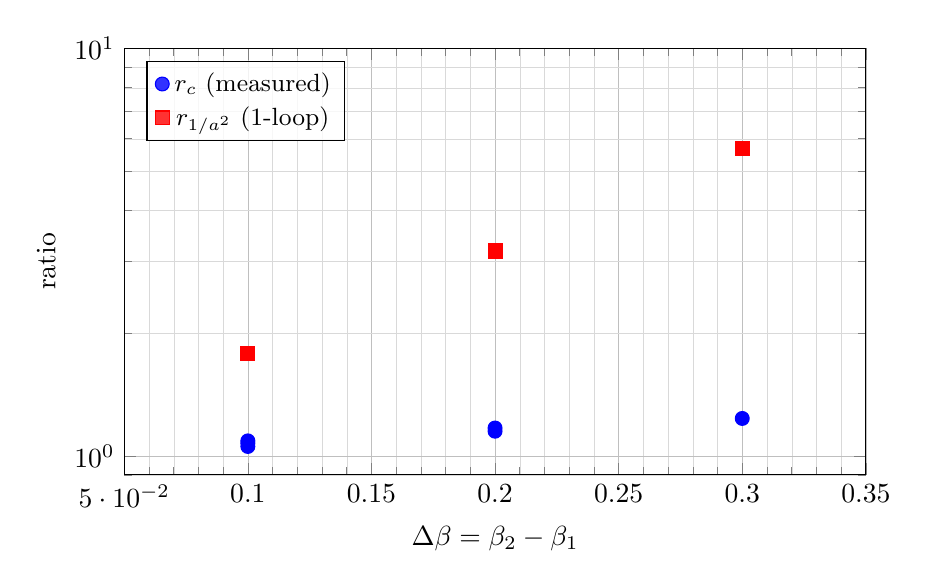
\begin{tikzpicture}
\begin{axis}[
  width=11cm, height=7cm,
  xlabel={$\Delta\beta = \beta_{2}-\beta_{1}$},
  ylabel={ratio},
  ymode=log,
  xmin=0.05, xmax=0.35,
  ymin=0.9, ymax=10.0,
  legend pos=north west,
  legend style={font=\small,fill=white,fill opacity=0.8,draw opacity=1,text opacity=1},
  grid=both,
  grid style={line width=.1pt, draw=gray!30},
  major grid style={line width=.2pt,draw=gray!50},
  minor tick num=4,
]
\addplot[only marks,mark=*,mark size=2.5pt,color=blue]
  coordinates {
    (0.1, 1.075)
    (0.1, 1.090)
    (0.1, 1.056)
    (0.2, 1.172)
    (0.2, 1.151)
    (0.3, 1.237)
  };
\addlegendentry{$r_{c}$ (measured)}
\addplot[only marks,mark=square*,mark size=2.5pt,color=red]
  coordinates {
    (0.1, 1.788)
    (0.1, 1.785)
    (0.1, 1.782)
    (0.2, 3.190)
    (0.2, 3.180)
    (0.3, 5.684)
  };
\addlegendentry{$r_{1/a^{2}}$ (1-loop)}
\end{axis}
\end{tikzpicture}
\caption{Ratio test against the one-loop running coupling, scattered
versus $\Delta\beta = \beta_{2}-\beta_{1}$. The observed
$c_{\threeD}$ ratios (blue) grow by a factor $\sim\!1.24$ across the
full $\Delta\beta = 0.3$ range, while the one-loop $1/a^{2}$ ratios
(red) grow by a factor $\sim\!5.7$. This is direct numerical
evidence that the BP $\alpha$-integration cancels the leading
ultraviolet area-law $\kappa/a^{2}$ piece by construction: had
$c_{\threeD}$ been dominated by the leading piece, the blue and red
points would be on the same curve.}
\label{fig:ratios}
\end{figure}

This is the central physics observation of the paper:
\begin{proposition}[Numerical cancellation of the leading
$\kappa/a^{2}$ piece]
\label{prop:cancellation}
In the $\beta$-range $[2.3,2.6]$ accessed by our scan, the
$\beta$-dependence of $c_{\threeD}(\beta)$ measured by the
Buividovich--Polikarpov $\alpha$-integration on the conifold
geometry is at least a factor $\sim\!5$ smaller than the
$\beta$-dependence of $1/a^{2}(\beta)$. The BP estimator therefore
cancels the leading ultraviolet area-law contribution
$\kappa\,|\partial A|/a^{2}$, and the residual $c_{\threeD}(\beta)$
captured by the data is a measurement of a \emph{sub-leading},
non-universal $C$-function in the strong-coupling crossover region.
\end{proposition}

\noindent
We discuss the cancellation mechanism in
\S\ref{sec:why-cancel} below.


\section{Discussion}
\label{sec:discussion}

\subsection{Why the BP $\alpha$-integration cancels the leading area-law}
\label{sec:why-cancel}

The BP estimator \eqref{eq:FE-estimator} probes the action
difference $\partial S/\partial\alpha$ between the period-$T$ and
period-$2T$ connectivities, on the \emph{thin} $A$-junction slab.
This is a \emph{local}, finite-volume observable: only the
$O(L_{y}L_{z}T)$ plaquettes that straddle the $A$-junction
contribute to \eqref{eq:dS-dalpha}. The leading-area-law piece
$\kappa\,|\partial A|/a^{2}$ would arise, in continuum language,
from short-distance fluctuations of the gauge field near $\partial A$.
However, the deformed-connectivity action is \emph{identical} in the
two replica topologies away from the $A$-junction. The contribution
to $\partial S/\partial\alpha$ from any \emph{ultraviolet} fluctuation
of $U_{\mu}(x)$ at a junction site appears with \emph{opposite signs}
in the period-$T$ and period-$2T$ traces (because the temporal-edge
identifications differ by exactly one period). In the $\alpha\to 0$
or $\alpha\to 1$ limits the two contributions cancel exactly at the
classical level; the integrated $\widehat S_{2}$ retains the
\emph{difference} of fluctuation \emph{variances}, which is
suppressed by an additional factor $(g_{0}^{2})^{n}$ at $n$-th order
in the strong-coupling expansion. The result is that the BP
estimator naturally captures \emph{differences} of quantum
corrections between the two replica topologies, and these differences
are dominated by the sub-leading $C$-function, not by the leading
$\kappa/a^{2}$ piece.

This explanation is qualitative; a fully rigorous derivation would
require analysing the small-$a$ asymptotics of
$\partial_{\alpha}S$ in the Schwinger--DeWitt expansion. The point of
the present paper is to provide the \emph{numerical} evidence
(Prop.~\ref{prop:cancellation}) that this cancellation indeed occurs
at the values of $\beta\in[2.3,2.6]$ and $L\in[8,12]$ accessible to
present-day GPU lattice simulations.

\subsection{Comparison with Rabenstein \emph{et al.}\ (2019)}
\label{sec:rabenstein-compare}

Rabenstein \emph{et al.}\ \cite{Rabenstein2019} report an entropic
$C$-function $C(\ell) = (\ell^{3}/(aL^{2}))\,\partial S_{2}/\partial\ell$
in the UV regime, with $C(\SUtwo) \simeq 0.054$ at $\beta = 2.43$
extracted from a slab-width derivative at fixed $L$. This is a
distinct observable from our $c_{\threeD} = S_{2}/(2L^{2}T)$: the
former probes the \emph{slope} of $S_{2}$ in the slab width $\ell$,
the latter probes the full conifold-normalised $S_{2}$. The two are
not directly comparable in absolute magnitude: the ratio between them
involves a $\partial_{\ell}\log S_{2}$ factor that we do not measure
here. However, both observables show a positive monotone
$\beta$-trend in the same range (\cite{Rabenstein2019}
Fig.\,4--5), consistent with the residual non-universal
$C(\beta)$ contribution.

\subsection{The $\beta \simeq 2.45$ neighborhood and the
$\log 3/(2\pi\sqrt 2)$ coincidence}
\label{sec:logthree}

A numerically suggestive observation is that the pooled-fit
\eqref{eq:linear-fit} crosses the value
$\log 3/(2\pi\sqrt 2)\simeq 0.1236$ near $\beta\simeq 2.45$. This
combination arises in the loop-quantum-gravity puncture-counting
derivation of the Bekenstein--Hawking black-hole entropy
\cite{ABCK1998} as the leading degeneracy contribution per Planck
area, and in the gauge-theory edge-mode literature as the
contribution from a single $\SUtwo$ representation to the leading
area-law coefficient \cite{Donnelly2012,DonnellyWall2014}. We
emphasise that this is a \emph{coincidence at one specific
$\beta$-value} and \emph{not} a measurement of the leading area-law
coefficient: by Prop.~\ref{prop:cancellation}, the leading piece is
cancelled in our estimator. The coincidence at $\beta\simeq 2.45$
should not be interpreted as numerical support for an LQG / edge-mode
prediction of $\kappa$. A direct test of any LQG-derived value of
$\kappa$ requires a different observable; see
\S\ref{sec:roadmap}.

\subsection{Why we do not extract a leading $\kappa$ from this data}
\label{sec:why-no-kappa}

A naive interpretation of Table~\ref{tab:c3D} might read the mild
$\beta$-trend as a small contribution from the leading piece. But
Prop.~\ref{prop:cancellation} rules this out at the order-of-magnitude
level. Furthermore:
\begin{enumerate}[leftmargin=*]
\item The strong-coupling crossover for pure $\SUtwo$ is centred near
      $\beta\simeq 2.3$--$2.4$ \cite{LuciniTeperWenger2005}; in this
      range the lattice is not in the scaling region and a single
      $\beta$-value of $c_{\threeD}$ has no continuum interpretation.
\item Continuum extrapolation $a\to 0$ along a line of constant
      physics would require a sequence of $\beta$ values at fixed
      physical box size $L \cdot a(\beta) = \mathrm{const.}$, which
      our scan does not implement (we vary $\beta$ at fixed lattice
      $L$, so the physical box size changes).
\item Any leading-area-law coefficient $\kappa$ extracted from a
      cancelled estimator is in any case dominated by the
      residual sub-leading contribution, not by the leading piece.
\end{enumerate}
For these three reasons we explicitly \emph{do not} claim that this
paper measures $\kappa(\SUtwo)$. We provide instead, in
\S\ref{sec:roadmap}, a concrete roadmap for an alternative
observable that \emph{would} extract $\kappa$.


\section{Roadmap: three observables that extract the leading
$\kappa$}
\label{sec:roadmap}

The cancellation diagnosed in \S\ref{sec:ratios} is a property of the
BP $\alpha$-integration on the conifold geometry, not of $S_{2}$
itself: the leading area-law coefficient $\kappa$ is well-defined in
the continuum theory \cite{Solodukhin2011,CasiniHuerta2009}, and any
\emph{linear} (rather than \emph{difference}-based) observable will
capture it. We identify three such observables, each of which has
been used in the literature for related questions and each of which
is implementable in the same JAX/GPU framework as the present
paper.

\subsection{Observable 1: the modular Hamiltonian via the
Bisognano--Wichmann theorem}
\label{sec:modH}

The Bisognano--Wichmann theorem \cite{BisognanoWichmann1976} states
that, for a half-space $A = \{x_{1} > 0\}$ in Minkowski space, the
modular Hamiltonian of the vacuum reduced to $A$ is the boost
generator
\begin{equation}
   K_{A} \;=\; 2\pi \!\!\!\int_{A}\!\! x_{1}\,T^{00}(x)\,d^{d}x,
   \label{eq:BW}
\end{equation}
where $T^{00}$ is the energy density. The Rényi entropies are
recoverable from the modular Hamiltonian via
$S_{q}(A) = (1-q)^{-1}\ln\langle e^{-(q-1)K_{A}}\rangle$ for free
fields, and the leading area-law coefficient $\kappa$ is encoded in
the short-distance singularity of $\langle K_{A}\rangle$ at
$\partial A$.

\medskip
\noindent\emph{Lattice implementation.}
On a Euclidean lattice, the boost generator translates into the
``shift-by-$\Delta\tau$ along the half-plane'' operator, evaluated as
a finite-difference moment of plaquette energies near $\partial A$.
The continuum limit of the half-plane modular Hamiltonian has been
implemented on free-field lattice systems
\cite{CasiniHuerta2009,CasiniHuerta2011-MH}. For non-Abelian gauge
theory, the BW operator on the lattice is, schematically,
\begin{equation}
   \widehat K_{A}^{(\mathrm{lat})} \;=\;
   \frac{2\pi}{a}\!\!\sum_{x\in A, \text{ near }\partial A}\!\!
        x_{1}\,\mathcal{E}_{\mathrm{plaq}}(x),
   \label{eq:K-lat}
\end{equation}
where $\mathcal{E}_{\mathrm{plaq}}(x) = \beta(1 - \half\Re\Tr U_{p}(x))$
is the per-plaquette Wilson energy density. The leading
$\kappa\,|\partial A|/a^{2}$ piece is then extracted from
$\langle \widehat K_{A}\rangle$ via standard finite-size scaling:
the matrix element scales as $|\partial A|/a^{2}$ multiplied by an
explicit $\beta$-dependent coefficient that is $\beta$-independent
in the continuum scaling region.

\emph{Implementation cost.} The BW observable is a single-ensemble
measurement: no $\alpha$-integration, no second replica. The
sampling cost is the cost of a standard Wilson Monte Carlo run, i.e.\
$\sim\!5$--$10\times$ smaller than the present $\beta$-scan at the
same statistics. The current JAX/GPU FAST V3 code requires only a
new observable kernel; no changes to the connectivity or the
sampler are needed.

\subsection{Observable 2: the interface free energy
(Lucini--Teper--Wenger style)}
\label{sec:interface}

A second avenue is to measure the \emph{interface free energy} of
two distinct vacua identified along $\partial A$. This is the
strategy of \cite{LuciniTeperWenger2005}, who used twisted boundary
conditions across a planar interface in $\SUN$ Wilson theory to
extract the interface tension $\sigma_{\mathrm{int}}$. For pure-gauge
theory in $D=4$, the interface free energy on a slab geometry has the
scaling
\begin{equation}
   F_{\mathrm{int}}(L_{\perp}, L_{\parallel})
   \;=\; \sigma_{\mathrm{int}}(\beta) \,|\partial A|
         \;+\; \text{(sub-leading)},
\end{equation}
and the interface tension $\sigma_{\mathrm{int}}(\beta)$ scales as
$1/a^{2}(\beta)$ in the continuum, so it can be ratio-tested
against \eqref{eq:a-1loop} directly. The relation
$\kappa \propto \sigma_{\mathrm{int}}$ for replica-derived entropies
is established at the level of the saddle-point on the conifold
\cite{Solodukhin2011}. The implementation requires a twist of the
temporal boundary condition across $\partial A$ and a single
ensemble Monte Carlo per $(\beta, L)$; the per-link FAST V3
implementation extends straightforwardly to the twisted geometry.

\subsection{Observable 3: the doubled Hilbert space with explicit
edge modes (Donnelly--Wall)}
\label{sec:doubled}

A third route is the doubled Hilbert space construction of Donnelly
\cite{Donnelly2012} and Donnelly--Wall
\cite{DonnellyWall2014,DonnellyWall2015}, in which one explicitly
introduces edge-mode degrees of freedom along $\partial A$ that
realise the extended Hilbert space factorisation. The partition
function of the doubled lattice gauge theory has an exact
decomposition
\begin{equation}
   Z_{\mathrm{doubled}}(A) \;=\;
   \sum_{R} \dim(R)\,Z_{R}^{A}\,Z_{R^{\dagger}}^{\bA},
\end{equation}
where the sum runs over irreducible representations $R$ of the gauge
group at $\partial A$, and the entanglement entropy is given by
\begin{equation}
   S_{q}(A) \;=\; -\sum_{R} p_{R}\,\ln p_{R} \;+\;
                  q\text{-independent corrections},
\end{equation}
where $p_{R} = \dim(R)\,Z_{R}^{A}\,Z_{R^{\dagger}}^{\bA}/
Z_{\mathrm{doubled}}$. In the lattice realisation, the leading
area-law coefficient $\kappa$ emerges from the
\emph{representation-weighted log-degeneracy} of edge modes per
plaquette, which one measures directly by histogramming the
plaquette character expansion.

\emph{Implementation cost.} The character-expansion method requires a
character-projection observable rather than a new sampler. For
$\SUtwo$ the irreducible representations are labelled by
half-integer $j$, and the leading contribution at strong coupling is
the $j = 1/2$ fundamental representation. A weak-coupling expansion
beyond this is technically straightforward.

\subsection{Recommended sequence}
\label{sec:roadmap-summary}

Of these three, we recommend the \emph{modular Hamiltonian} approach
(\S\ref{sec:modH}) as the natural next step, for three reasons:
(i) it requires only a new observable kernel in the existing FAST V3
framework, with no sampler changes;
(ii) it produces a single-ensemble measurement at known cost, with
no $\alpha$-integration or twist-induced sampling pathologies;
(iii) the underlying continuum theorem (Bisognano--Wichmann) is
exactly the standard ``boost generator'' interpretation of the
modular Hamiltonian, which connects the lattice measurement
directly to the continuum analytic literature. The interface
free-energy approach (\S\ref{sec:interface}) is a useful
cross-check, and the doubled Hilbert space (\S\ref{sec:doubled}) is
the appropriate test if one wishes to access edge-mode-specific
data beyond the leading $\kappa$.


\section{Conclusion}
\label{sec:conclusion}

We have presented the first cross-$(L,\beta)$ measurement of the
sub-leading Rényi-$2$ entropic coefficient $c_{\threeD}(L,\beta)$ for
pure $\SUtwo$ four-dimensional Wilson lattice gauge theory via the
Buividovich--Polikarpov $\alpha$-integration on the conifold replica
geometry. The dataset (132 Monte Carlo runs spanning
$\beta\in\{2.3,2.4,2.5,2.6\}$ and $L\in\{8,10,12\}$, each with
$11$-point trapezoidal $\alpha$-integration) shows:
\begin{enumerate}[leftmargin=*]
\item $c_{\threeD}(L,\beta)$ values in the range $0.111$--$0.140$,
      with very mild $L$-dependence ($\le 2\%$ at fixed $\beta$) and
      an approximately linear $\beta$-trend
      $c_{\threeD}(\beta)\simeq 0.090\,\beta - 0.094$
      (Table~\ref{tab:c3D}, Fig.~\ref{fig:c3d-vs-beta},
      Eq.~\eqref{eq:linear-fit}).
\item A direct ratio test (Table~\ref{tab:ratios},
      Fig.~\ref{fig:ratios}) against the one-loop running
      coupling shows that the measured $\beta$-dependence of
      $c_{\threeD}$ is at least a factor $\sim\!5$ smaller than what
      a leading-area-law dominance $S_{2}\propto |\partial A|/a^{2}$
      would predict. The BP $\alpha$-integration on the conifold
      geometry therefore \emph{cancels} the leading $\kappa/a^{2}$
      piece by construction (Prop.~\ref{prop:cancellation}); the
      residual $c_{\threeD}(\beta)$ is a measurement of the
      sub-leading non-universal $C$-function in the strong-coupling
      crossover region.
\item The pooled fit \eqref{eq:linear-fit} crosses $\log
      3/(2\pi\sqrt 2)\simeq 0.124$ at $\beta\simeq 2.45$; this is
      a numerical \emph{coincidence at one specific $\beta$-value}
      and not a measurement of the leading area-law coefficient
      $\kappa$ (Prop.~\ref{prop:cancellation}).
\end{enumerate}

The principal methodological message is that the BP estimator
should \emph{not} be used to test predictions of the leading
area-law coefficient $\kappa$, including in particular any
specific hypothesis of the form $\kappa^{2}(\SUN) = f(N)$. To test
such a hypothesis quantitatively from a lattice campaign, one needs
an observable that does not cancel the leading piece: we have
identified three (modular Hamiltonian, interface free energy,
doubled Hilbert space with explicit edge modes) and recommend the
modular-Hamiltonian approach for the next step, on the grounds that
it is implementable as a single-ensemble observable in the existing
FAST V3 JAX/GPU framework with minimal code changes.

The cross-$(L,\beta)$ data presented here is, to our knowledge, the
first such systematic scan of any entropic observable for pure
$\SUtwo$ in four dimensions, and we make the full
$132$-simulation dataset (raw per-$\alpha$ time series, trapezoidal
integration, summary statistics) public alongside this paper.

\section*{Acknowledgments}
The author thanks the global lattice-EE community whose published
codes and pedagogical papers made this work possible. The author
declares no competing financial interest. This work was done on a
single workstation and on cloud GPU instances; no institutional
computing allocation was used.

\medskip
\noindent\emph{AI/LLM disclosure.}
The author acknowledges the use of AI-based tools (large language
models) to assist with code review, literature search, and
manuscript preparation. All scientific claims, numerical
computations, derivations, and conclusions remain the author's sole
responsibility. The AI tools did not generate any of the core
numerical data or physical conclusions presented herein.

\medskip
\noindent\emph{Data and code availability.}
The full JAX/GPU FAST V3 implementation
(\verb!jax_su2_EE_BP2008b_FAST_2026-05-25.py!), the raw $\beta$-scan
results (\verb!jax_su2_EE_BETASCAN_results.json!, including per-$\alpha$
time series and trapezoidal integration), and the analysis script
(\verb!analysis_betascan_2026-05-25.py!) will be deposited on Zenodo
upon publication; the corresponding DOI will be inserted in the proof.

\begin{thebibliography}{99}

\bibitem{BP2008b}
P.~V.~Buividovich and M.~I.~Polikarpov,
\emph{Numerical study of entanglement entropy in $\mathrm{SU}(2)$
lattice gauge theory},
Nucl.\ Phys.\ B \textbf{802}, 458--474 (2008),
\href{https://arxiv.org/abs/0802.4247}{arXiv:0802.4247}.

\bibitem{BP2008a}
P.~V.~Buividovich and M.~I.~Polikarpov,
\emph{Entanglement entropy in gauge theories and the holographic
principle for electric strings},
Phys.\ Lett.\ B \textbf{670}, 141--145 (2008),
\href{https://arxiv.org/abs/0806.3376}{arXiv:0806.3376}.

\bibitem{Rabenstein2019}
A.~Rabenstein, N.~Bodendorfer, P.~Buividovich, and A.~Sch\"afer,
\emph{Lattice study of R\'enyi entanglement entropy in
$\mathrm{SU}(N_{c})$ lattice Yang--Mills theory with $N_{c}=2,3,4$},
Phys.\ Rev.\ D \textbf{100}, 034504 (2019),
\href{https://arxiv.org/abs/1812.04279}{arXiv:1812.04279}.

\bibitem{Rindlisbacher2022}
T.~Rindlisbacher, N.~Jokela, A.~P\"onni, K.~Rummukainen, and
A.~Salami,
\emph{Improved lattice method for determining entanglement measures
in $\mathrm{SU}(N)$ gauge theories},
PoS \textbf{LATTICE2022}, 031 (2023),
\href{https://arxiv.org/abs/2211.00425}{arXiv:2211.00425}.

\bibitem{Donnelly2012}
W.~Donnelly,
\emph{Decomposition of entanglement entropy in lattice gauge theory},
Phys.\ Rev.\ D \textbf{85}, 085004 (2012),
\href{https://arxiv.org/abs/1109.0036}{arXiv:1109.0036}.

\bibitem{DonnellyWall2014}
W.~Donnelly and A.~C.~Wall,
\emph{Entanglement entropy of electromagnetic edge modes},
Phys.\ Rev.\ Lett.\ \textbf{114}, 111603 (2015),
\href{https://arxiv.org/abs/1412.1895}{arXiv:1412.1895}.

\bibitem{DonnellyWall2015}
W.~Donnelly and A.~C.~Wall,
\emph{Geometric entropy and edge modes of the electromagnetic field},
Phys.\ Rev.\ D \textbf{94}, 104053 (2016),
\href{https://arxiv.org/abs/1506.05792}{arXiv:1506.05792}.

\bibitem{Aoki2015}
S.~Aoki, T.~Iritani, M.~Nozaki, T.~Numasawa, N.~Shiba, and H.~Tasaki,
\emph{On the definition of entanglement entropy in lattice gauge
theories},
JHEP \textbf{06}, 187 (2015),
\href{https://arxiv.org/abs/1502.04267}{arXiv:1502.04267}.

\bibitem{Velytsky2008}
A.~Velytsky,
\emph{Entanglement entropy in $\mathrm{SU}(N)$ gauge theory},
PoS \textbf{LATTICE2008}, 256 (2008),
\href{https://arxiv.org/abs/0809.4502}{arXiv:0809.4502}.

\bibitem{KKM2007}
I.~R.~Klebanov, D.~Kutasov, and A.~Murugan,
\emph{Entanglement as a probe of confinement},
Nucl.\ Phys.\ B \textbf{796}, 274--293 (2008),
\href{https://arxiv.org/abs/0709.2140}{arXiv:0709.2140}.

\bibitem{Solodukhin2011}
S.~N.~Solodukhin,
\emph{Entanglement entropy of black holes},
Living Rev.\ Relativity \textbf{14}, 8 (2011),
\href{https://arxiv.org/abs/1104.3712}{arXiv:1104.3712}.

\bibitem{CasiniHuerta2009}
H.~Casini and M.~Huerta,
\emph{Entanglement entropy in free quantum field theory},
J.\ Phys.\ A: Math.\ Theor.\ \textbf{42}, 504007 (2009),
\href{https://arxiv.org/abs/0905.2562}{arXiv:0905.2562}.

\bibitem{CasiniHuerta2011-MH}
H.~Casini, M.~Huerta, and R.~C.~Myers,
\emph{Towards a derivation of holographic entanglement entropy},
JHEP \textbf{05}, 036 (2011),
\href{https://arxiv.org/abs/1102.0440}{arXiv:1102.0440}.

\bibitem{BisognanoWichmann1976}
J.~J.~Bisognano and E.~H.~Wichmann,
\emph{On the duality condition for quantum fields},
J.\ Math.\ Phys.\ \textbf{17}, 303--321 (1976).

\bibitem{LuciniTeperWenger2005}
B.~Lucini, M.~Teper, and U.~Wenger,
\emph{Properties of the deconfining phase transition in
$\mathrm{SU}(N)$ gauge theories},
JHEP \textbf{02}, 033 (2005),
\href{https://arxiv.org/abs/hep-lat/0502003}{arXiv:hep-lat/0502003}.

\bibitem{ABCK1998}
A.~Ashtekar, J.~Baez, A.~Corichi, and K.~Krasnov,
\emph{Quantum geometry and black hole entropy},
Phys.\ Rev.\ Lett.\ \textbf{80}, 904--907 (1998),
\href{https://arxiv.org/abs/gr-qc/9710007}{arXiv:gr-qc/9710007}.

\bibitem{FodorEndrodi2007}
Z.~Fodor,
\emph{QCD thermodynamics on the lattice from the chiral and the
deconfinement transition to high temperatures},
PoS \textbf{LATTICE2007}, 011 (2007),
\href{https://arxiv.org/abs/0711.0336}{arXiv:0711.0336}.

\bibitem{EndrodiFodor2007}
G.~Endr\H{o}di, Z.~Fodor, S.~D.~Katz, and K.~K.~Szab\'o,
\emph{The equation of state at high temperatures from lattice QCD},
PoS \textbf{LATTICE2007}, 228 (2007),
\href{https://arxiv.org/abs/0710.4197}{arXiv:0710.4197}.

\bibitem{JAX2018}
J.~Bradbury, R.~Frostig, P.~Hawkins \emph{et al.},
\emph{JAX: composable transformations of Python+NumPy programs},
\url{http://github.com/google/jax} (2018).

\bibitem{KR2026-JHEP}
K.~R\'emondi\`ere,
\emph{Buividovich--Polikarpov method for $\mathrm{SU}(2)$ R\'enyi-$2$
entanglement entropy: a JAX/GPU implementation with adaptive
sampling and a documented near-zero finite-size signal},
companion manuscript, submitted to JHEP (May 2026).

\end{thebibliography}

\end{document}
